\chapter{Methods}\label{chap:methods}

This chapter describes the mass-moving purification algorithm and our implementation for XGBoost depth-2 ensembles.

\section{Mass-Moving Purification Algorithm}\label{sec:mass-moving}

The purification algorithm enforces the weighted slice mean-zero constraints (\cref{eq:row-constraint,eq:col-constraint}) by iteratively ``moving mass'' from higher-order tensors to lower-order tensors.

\subsection{Purify-Matrix: A Single Interaction Tensor}

For a pairwise interaction matrix $\mathbf{F}_{ij} \in \mathbb{R}^{B_i \times B_j}$ with marginal weight vectors $\mathbf{w}_i \in \mathbb{R}^{B_i}$ and $\mathbf{w}_j \in \mathbb{R}^{B_j}$, each sweep proceeds as follows:
\begin{enumerate}
    \item \textbf{Row sweep} (enforcing the row constraint): for each row $r = 1, \ldots, B_i$:
    \begin{enumerate}
        \item Compute the weighted mean across columns: $\bar{m}_r = \frac{\sum_{k=1}^{B_j} \mathbf{F}_{ij}[r, k] \cdot w_j[k]}{\sum_{k=1}^{B_j} w_j[k]}$.
        \item Subtract from the interaction row: $\mathbf{F}_{ij}[r, k] \leftarrow \mathbf{F}_{ij}[r, k] - \bar{m}_r$ for all $k$.
        \item Add to the main effect of $X_i$: $f_i[r] \leftarrow f_i[r] + \bar{m}_r$.
    \end{enumerate}
    \item \textbf{Column sweep} (enforcing the column constraint): for each column $c = 1, \ldots, B_j$:
    \begin{enumerate}
        \item Compute the weighted mean across rows: $\bar{m}_c = \frac{\sum_{k=1}^{B_i} \mathbf{F}_{ij}[k, c] \cdot w_i[k]}{\sum_{k=1}^{B_i} w_i[k]}$.
        \item Subtract from the interaction column: $\mathbf{F}_{ij}[k, c] \leftarrow \mathbf{F}_{ij}[k, c] - \bar{m}_c$ for all $k$.
        \item Add to the main effect of $X_j$: $f_j[c] \leftarrow f_j[c] + \bar{m}_c$.
    \end{enumerate}
    \item Repeat sweeps until $\max_{r,c}(|\bar{m}_r|, |\bar{m}_c|) \leq \varepsilon$.
\end{enumerate}

This is a Gauss--Seidel-style iteration: updating rows changes the column means, so the process iterates.
The key invariant is that $F(\mathbf{x})$ is unchanged after each step, since the subtracted mass is added to a lower-order term.
If $\sum_k w_j[k] = 0$ for a particular slice, the weighted mean is undefined; we treat this as $\bar{m} = 0$ (no mass is moved).

\subsection{Worked Example}

\Cref{fig:mass-moving-walkthrough} illustrates one row sweep on a $3 \times 3$ interaction matrix with uniform weights.

\begin{figure}[H]
\centering
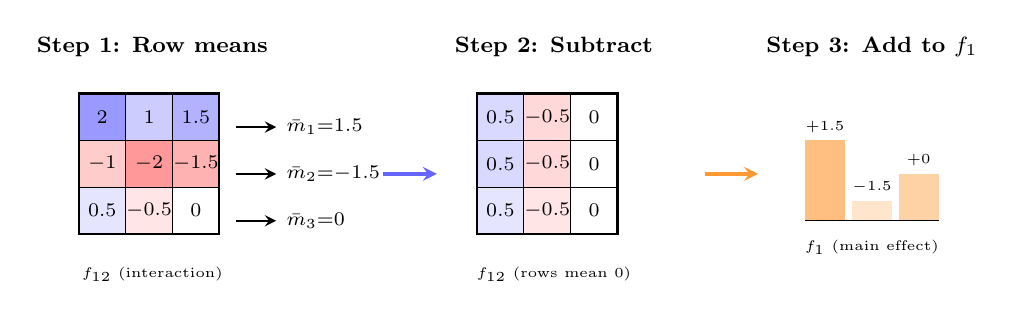
\begin{tikzpicture}[scale=0.85,
  arr/.style={->,thick,>=stealth}]

  % Step 1: Interaction tensor with non-zero row means
  \node[font=\footnotesize\bfseries] at (1.05,3.2) {Step 1: Row means};
  \begin{scope}[shift={(-0.05,0.4)}]
    \fill[blue!40] (0,1.4) rectangle (0.7,2.1); \node[font=\scriptsize] at (0.35,1.75) {2};
    \fill[blue!20] (0.7,1.4) rectangle (1.4,2.1); \node[font=\scriptsize] at (1.05,1.75) {1};
    \fill[blue!30] (1.4,1.4) rectangle (2.1,2.1); \node[font=\scriptsize] at (1.75,1.75) {1.5};
    \fill[red!20] (0,0.7) rectangle (0.7,1.4); \node[font=\scriptsize] at (0.35,1.05) {$-$1};
    \fill[red!40] (0.7,0.7) rectangle (1.4,1.4); \node[font=\scriptsize] at (1.05,1.05) {$-$2};
    \fill[red!30] (1.4,0.7) rectangle (2.1,1.4); \node[font=\scriptsize] at (1.75,1.05) {$-$1.5};
    \fill[blue!10] (0,0) rectangle (0.7,0.7); \node[font=\scriptsize] at (0.35,0.35) {0.5};
    \fill[red!10] (0.7,0) rectangle (1.4,0.7); \node[font=\scriptsize] at (1.05,0.35) {$-$0.5};
    \fill[white] (1.4,0) rectangle (2.1,0.7); \draw (1.4,0) rectangle (2.1,0.7); \node[font=\scriptsize] at (1.75,0.35) {0};
    \draw[thick] (0,0) rectangle (2.1,2.1);
    \draw (0,0.7) -- (2.1,0.7); \draw (0,1.4) -- (2.1,1.4);
    \draw (0.7,0) -- (0.7,2.1); \draw (1.4,0) -- (1.4,2.1);
  \end{scope}
  \node[font=\tiny] at (1.05,-0.2) {$f_{12}$ (interaction)};
  \draw[arr] (2.3,2.0) -- (2.9,2.0) node[right,font=\scriptsize] {$\bar{m}_1{=}1.5$};
  \draw[arr] (2.3,1.3) -- (2.9,1.3) node[right,font=\scriptsize] {$\bar{m}_2{=}{-}1.5$};
  \draw[arr] (2.3,0.6) -- (2.9,0.6) node[right,font=\scriptsize] {$\bar{m}_3{=}0$};

  % Arrow to step 2
  \draw[arr,very thick,blue!60] (4.5,1.3) -- (5.3,1.3);

  % Step 2: Subtract means from rows
  \node[font=\footnotesize\bfseries] at (7.05,3.2) {Step 2: Subtract};
  \begin{scope}[shift={(5.9,0.4)}]
    \fill[blue!15] (0,1.4) rectangle (0.7,2.1); \node[font=\scriptsize] at (0.35,1.75) {0.5};
    \fill[red!15] (0.7,1.4) rectangle (1.4,2.1); \node[font=\scriptsize] at (1.05,1.75) {$-$0.5};
    \fill[white] (1.4,1.4) rectangle (2.1,2.1); \draw (1.4,1.4) rectangle (2.1,2.1); \node[font=\scriptsize] at (1.75,1.75) {0};
    \fill[blue!15] (0,0.7) rectangle (0.7,1.4); \node[font=\scriptsize] at (0.35,1.05) {0.5};
    \fill[red!15] (0.7,0.7) rectangle (1.4,1.4); \node[font=\scriptsize] at (1.05,1.05) {$-$0.5};
    \fill[white] (1.4,0.7) rectangle (2.1,1.4); \draw (1.4,0.7) rectangle (2.1,1.4); \node[font=\scriptsize] at (1.75,1.05) {0};
    \fill[blue!10] (0,0) rectangle (0.7,0.7); \node[font=\scriptsize] at (0.35,0.35) {0.5};
    \fill[red!10] (0.7,0) rectangle (1.4,0.7); \node[font=\scriptsize] at (1.05,0.35) {$-$0.5};
    \fill[white] (1.4,0) rectangle (2.1,0.7); \draw (1.4,0) rectangle (2.1,0.7); \node[font=\scriptsize] at (1.75,0.35) {0};
    \draw[thick] (0,0) rectangle (2.1,2.1);
    \draw (0,0.7) -- (2.1,0.7); \draw (0,1.4) -- (2.1,1.4);
    \draw (0.7,0) -- (0.7,2.1); \draw (1.4,0) -- (1.4,2.1);
  \end{scope}
  \node[font=\tiny] at (7.05,-0.2) {$f_{12}$ (rows mean 0)};

  % Arrow to step 3
  \draw[arr,very thick,orange!80] (9.3,1.3) -- (10.1,1.3);

  % Step 3: Add to main effect
  \node[font=\footnotesize\bfseries] at (11.8,3.2) {Step 3: Add to $f_1$};
  \begin{scope}[shift={(10.8,0.6)}]
    \fill[orange!50] (0,0) rectangle (0.6,1.2);
    \fill[orange!20] (0.7,0) rectangle (1.3,0.3);
    \fill[orange!35] (1.4,0) rectangle (2.0,0.7);
    \draw (0,0) -- (2.0,0);
    \node[font=\tiny] at (1.0,-0.4) {$f_1$ (main effect)};
    \node[font=\tiny] at (0.3,1.4) {+1.5};
    \node[font=\tiny] at (1.0,0.5) {$-$1.5};
    \node[font=\tiny] at (1.7,0.9) {+0};
  \end{scope}
\end{tikzpicture}
\caption[Visual walkthrough of one mass-moving sweep.]{One row sweep of the mass-moving algorithm on a $3 \times 3$ interaction matrix (uniform weights). Step~1: compute row means. Step~2: subtract from interaction. Step~3: add to $f_1$. The overall function $f_1(x_1) + f_{12}(x_1, x_2)$ is unchanged.}
\label{fig:mass-moving-walkthrough}
\end{figure}

\subsection{Purify-All: Processing All Tensors}

To purify a complete additive model, we process tensors in descending order of interaction order.
For depth-2 models: purify all pairwise interaction matrices first, then center all main effects (subtracting their weighted mean and adding it to the intercept).

\begin{algorithm}[ht]
\caption{Mass-moving purification (Purify-All)}\label{alg:purify-all}
\begin{algorithmic}[1]
\Require Tensors $\{T_u\}$ for all subsets $u$, weights $\{w_u\}$, tolerance $\varepsilon$
\Ensure Purified tensors satisfying slice mean-zero constraints
\State Sort keys $u$ by $|u|$ descending
\For{each $u$ in sorted order}
    \Repeat
        \State $\text{max\_residual} \leftarrow 0$
        \For{each axis $a$ corresponding to variable $i \in u$}
            \For{each slice along the other axes}
                \State $\bar{m} \leftarrow$ weighted mean of slice using $w_i$
                \State $T_u[\text{slice}] \leftarrow T_u[\text{slice}] - \bar{m}$
                \State $T_{u \setminus \{i\}}[\text{corresponding entry}] \leftarrow T_{u \setminus \{i\}}[\ldots] + \bar{m}$
                \State $\text{max\_residual} \leftarrow \max(\text{max\_residual}, |\bar{m}|)$
            \EndFor
        \EndFor
    \Until{$\text{max\_residual} \leq \varepsilon$}
\EndFor
\end{algorithmic}
\end{algorithm}

\subsection{Convergence Properties}

\citet{lengerich2020purifying} proved that for uniform or factored weight distributions, purification converges in a single pass (row sweeps do not alter column means).
For arbitrary positive weights, convergence to tolerance $\varepsilon$ requires $O(\log(M_0) - \log(\varepsilon))$ iterations.
\Cref{fig:convergence} confirms this empirically: uniform weights converge in one sweep; random weights reach $10^{-10}$ within 5--10 sweeps.

\begin{figure}[H]
\centering
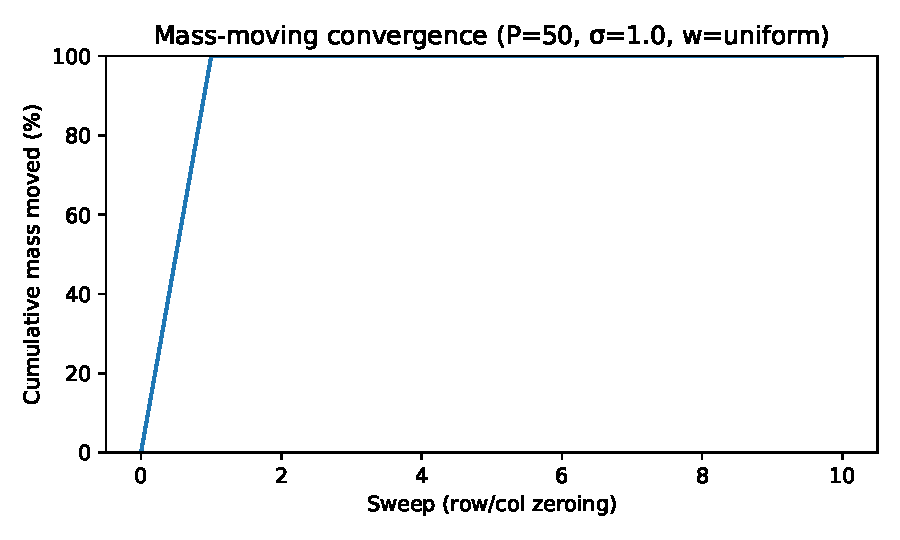
\includegraphics[width=0.48\textwidth]{convergence_uniform_sigma1.0.pdf}%
\hfill%
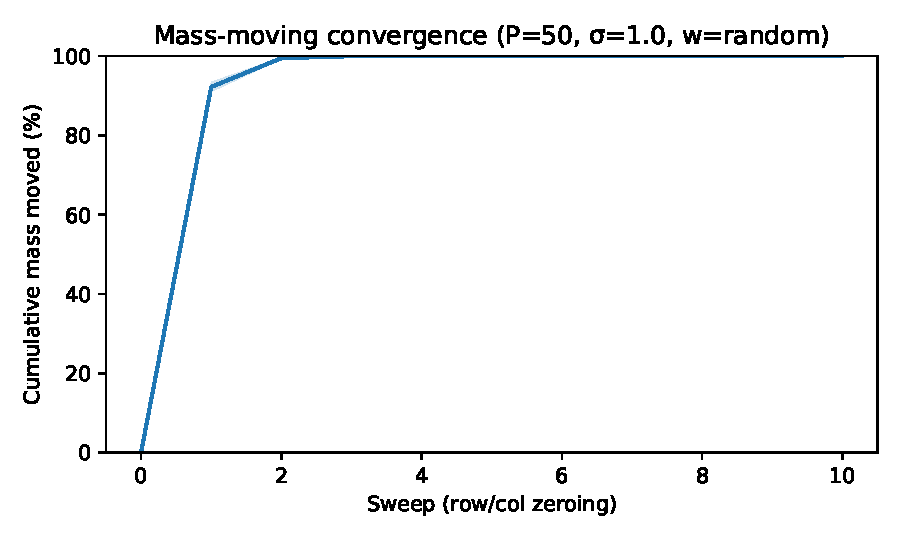
\includegraphics[width=0.48\textwidth]{convergence_random_sigma1.0.pdf}
\caption[Convergence of the mass-moving algorithm.]{Convergence on random $50 \times 50$ matrices ($\sigma = 1.0$). Left: uniform weights---one sweep. Right: random weights---exponential decay over 5--10 sweeps.}
\label{fig:convergence}
\end{figure}

\section{XGBoost Depth-2 Decomposition}\label{sec:xgb-decompose}

For an XGBoost model restricted to depth $\leq 2$, each root-to-leaf path uses at most two features, enabling exact decomposition into main effects and pairwise interactions.

\subsection{Binning}

The bin boundaries for each feature $x_j$ are defined by the union of all split thresholds across all trees, partitioning the axis into $K+1$ bins.
Each input is mapped to a bin index via $\text{searchsorted}$, matching XGBoost's ``left if $x < t$'' convention.

\subsection{Tensor Construction}

The ensemble is decomposed into:
\begin{itemize}
    \item An intercept $T_{()} = \text{base\_score}$.
    \item Main effect vectors $T_{(i)} \in \mathbb{R}^{B_i}$, from leaf paths using only feature $i$.
    \item Interaction matrices $T_{(i,j)} \in \mathbb{R}^{B_i \times B_j}$, from leaf paths using features $i$ and $j$.
\end{itemize}

For each tree, we extract all root-to-leaf paths; each path defines a rectangular region in bin space, and the leaf value is added to all tensor entries within that region.
A depth-2 tree can use up to three features across branches, but each path uses at most two, so the tree decomposes into pairwise interactions and main effects at the path level.

\subsection{Exactness}

This decomposition is exact:
\[
    F(\mathbf{x}) = T_{()} + \sum_i T_{(i)}[\text{bin}_i(\mathbf{x})] + \sum_{i<j} T_{(i,j)}[\text{bin}_i(\mathbf{x}), \text{bin}_j(\mathbf{x})]
\]
reproduces XGBoost's predictions exactly, verified in every experiment.

\section{Prediction Invariance}

Purification preserves predictions by construction: subtracting $\bar{m}$ from a row of $\mathbf{F}_{ij}$ and adding it to $f_i$ leaves
\[
    f_i[\text{bin}_i] + \mathbf{F}_{ij}[\text{bin}_i, \text{bin}_j] = (f_i[\text{bin}_i] + \bar{m}) + (\mathbf{F}_{ij}[\text{bin}_i, \text{bin}_j] - \bar{m}) = \text{unchanged}.
\]
We verify this empirically by checking $\max_{\mathbf{x}} |F_{\text{model}}(\mathbf{x}) - F_{\text{purified}}(\mathbf{x})| < 10^{-2}$.
